% CVPR 2023 Paper Template
% based on the CVPR template provided by Ming-Ming Cheng (https://github.com/MCG-NKU/CVPR_Template)
% modified and extended by Stefan Roth (stefan.roth@NOSPAMtu-darmstadt.de)

\documentclass[10pt,twocolumn,letterpaper]{article}
\usepackage{CJKutf8}
%%%%%%%%% PAPER TYPE  - PLEASE UPDATE FOR FINAL VERSION
%\usepackage[review]{cvpr}      % To produce the REVIEW version
\usepackage{cvpr}              % To produce the CAMERA-READY version
%\usepackage[pagenumbers]{cvpr} % To force page numbers, e.g. for an arXiv version

% Include other packages here, before hyperref.
\usepackage{graphicx}
\usepackage{amsmath}
\usepackage{amssymb}
\usepackage{booktabs}



% It is strongly recommended to use hyperref, especially for the review version.
% hyperref with option pagebackref eases the reviewers' job.
% Please disable hyperref *only* if you encounter grave issues, e.g. with the
% file validation for the camera-ready version.
%
% If you comment hyperref and then uncomment it, you should delete
% ReviewTempalte.aux before re-running LaTeX.
% (Or just hit 'q' on the first LaTeX run, let it finish, and you
%  should be clear).
\usepackage[pagebackref,breaklinks,colorlinks]{hyperref}


% Support for easy cross-referencing
\usepackage[capitalize]{cleveref}
\crefname{section}{Sec.}{Secs.}
\Crefname{section}{Section}{Sections}
\Crefname{table}{Table}{Tables}
\crefname{table}{Tab.}{Tabs.}


%%%%%%%%% PAPER ID  - PLEASE UPDATE
\def\cvprPaperID{*****} % *** Enter the CVPR Paper ID here
\def\confName{CVPR}
\def\confYear{2023}


\begin{document}

%%%%%%%%% TITLE - PLEASE UPDATE
\title{DeepFake Detection on Android}
\author{Q56121052 \begin{CJK*}{UTF8}{bsmi}黃書堯
\end{CJK*}\\
{\tt\small david070889@gmail.com}
% For a paper whose authors are all at the same institution,
% omit the following lines up until the closing ``}''.
% Additional authors and addresses can be added with ``\and'',
% just like the second author.
% To save space, use either the email address or home page, not both
}
\maketitle

%%%%%%%%% ABSTRACT
% \begin{abstract}
%    The ABSTRACT is to be in fully justified italicized text, at the top of the left-hand column, below the author and affiliation information.
%    Use the word ``Abstract'' as the title, in 12-point Times, boldface type, centered relative to the column, initially capitalized.
%    The abstract is to be in 10-point, single-spaced type.
%    Leave two blank lines after the Abstract, then begin the main text.
%    Look at previous CVPR abstracts to get a feel for style and length.
% \end{abstract}

\begin{abstract}
With the increasing proliferation of deepfakes, the need for effective detection mechanisms has become crucial. This paper presents the development of an Android application capable of detecting deepfakes using lightweight deep learning models. The application allows users to select or capture images, perform face detection, and determine the authenticity of faces. We compare the execution time and accuracy of various lightweight models trained on the FF++\cite{Rossler_2019_ICCV} dataset and investigate their generalizability across different datasets.
\end{abstract}
%%%%%%%%% BODY TEXT
\section{Introduction}
\label{sec:intro}
Over the past few years, the advancement of AI has surpassed our wildest imaginations, resulting in the invention of numerous groundbreaking tools. Deepfake technology stands out as one of these remarkable tools, revolutionizing the modern multimedia industry with its profound impact.

Fabrication and manipulation of digital images and videos are not new\cite{Farid2020}. However, due to its significant influence, Deepfake technology has gradually fallen into the wrong hands. More and more malicious users have exploited it for unlawful or nefarious purposes. In order to prevent the dissemination of misinformation throughout society via the internet, it is imperative to develop approaches for detecting whether images or videos have been manipulated\cite{9721302}.

Detecting deepfake content on mobile devices presents several challenges, making it a complex task for researchers. Firstly, the rapid advancement in artificial intelligence and machine learning algorithms has led to the creation of highly realistic and convincing fake images and videos. These sophisticated techniques can manipulate facial expressions, voices, and even body movements with such precision that distinguishing them from real content becomes difficult. 

Secondly, the vast diversity in human faces, expressions, and lighting conditions in videos adds another layer of complexity to the detection process. Algorithms must be trained on extensive and varied datasets to accurately identify anomalies. 

Thirdly, the detection models themselves require significant computational resources, making it challenging to deploy these models in mobile applications while balancing both performance and cost. Addressing these challenges requires a multifaceted approach, combining advances in AI research, ethical guidelines, and possibly regulatory measures to mitigate the impacts of deepfakes.

%-------------------------------------------------------------------------

\section{System framework}
\label{sec:formatting}
After conducting a thorough statistical analysis of the existing studies in the field of deepfake detection, Rana \etal~\cite{9721302} found that an overwhelming 77\% of the research have been concentrated on deep learning methodologies. Among these deep learning-based studies, a significant majority, constituting 78\%, have specifically utilized Convolutional Neural Networks (CNNs) as their detection frameworks.

Given this overwhelming trend towards CNNs, we decided that this project would primarily focus on leveraging CNN models developed with PyTorch\cite{paszke2019pytorch}.

Among the numerous CNN architectures available, special emphasis will be placed on exploring and implementing models based on limited resources suitable for mobile devices. PyTorch\cite{paszke2019pytorch} and PyTorch Mobile will be implemented on my phone with Snapdragon 7+ Gen2 CPU and 16GB RAM. The decision to base on these advanced architectures stems from their proven efficacy in various image recognition tasks and their computational ability on edge devices.


%-------------------------------------------------------------------------

\section{Dataset}
The FaceForensics++\cite{Rossler_2019_ICCV} dataset stands as a pivotal resource in the domain of digital forensics, particularly for training and evaluating deepfake detection models, it's a large-scale dataset of manipulations based on the classical computer graphics-based methods
Face2Face\cite{Thies_2016_CVPR} and FaceSwap as well as the learning-based approaches DeepFakes, NeuralTexture\cite{10.1145/3306346.3323035} and FaceShifter\cite{li2020faceshifter}. It features a vast collection of video sequences, with thousands of videos that have been expertly altered using these sophisticated manipulation techniques, paired with their original, unaltered versions. Notably, the dataset's diversity — in terms of lighting conditions, facial expressions, and backgrounds — makes it an excellent platform for rigorously testing deepfake detection algorithms across a spectrum of scenarios.

To evaluate the generalizability of our models, we selected another well-known dataset, Celeb-DF-v2.\cite{li2020celebdf}. Celeb-DF-v2\cite{li2020celebdf} is a challenging deepfake dataset that contains high-quality deepfake videos created using improved synthesis techniques, making it more difficult to detect compared to other datasets. It consists of real and fake videos of celebrities, offering a diverse range of facial expressions, lighting conditions, and background scenes. Testing our models on Celeb-DF-v2\cite{li2020celebdf} allows us to assess their robustness and effectiveness in detecting deepfakes in real-world scenarios, ensuring that the models can maintain high performance even when faced with previously unseen data and different manipulation techniques.

\begin{figure*}
  \centering
   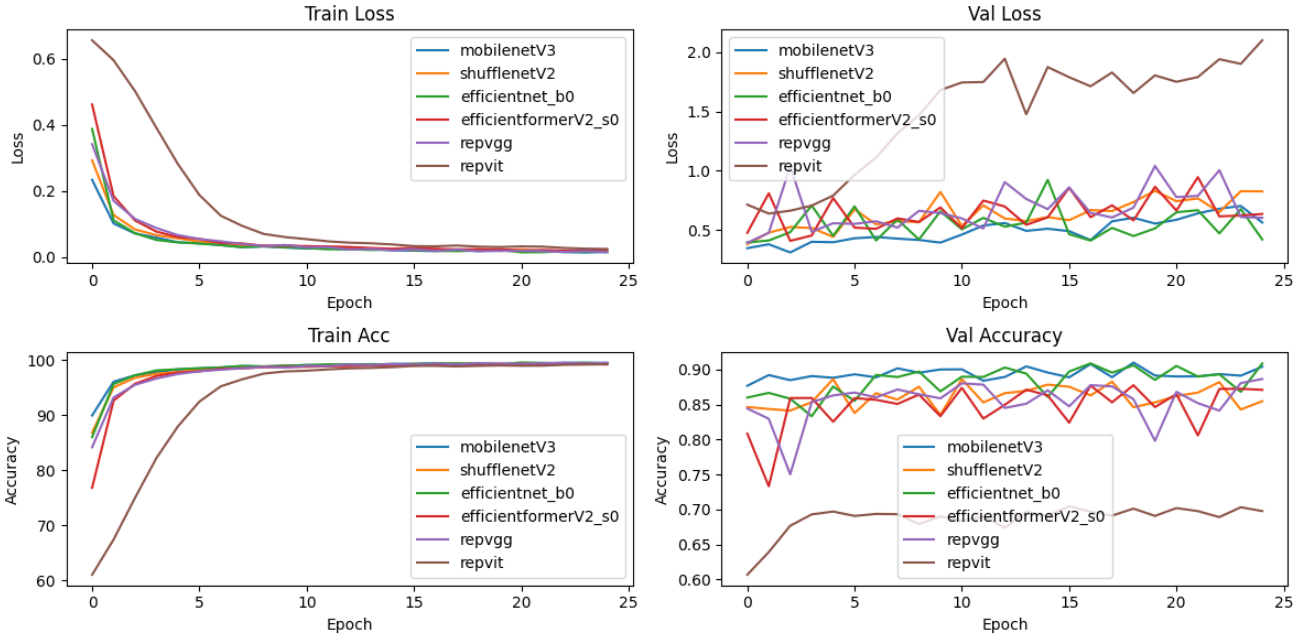
\includegraphics[width=0.8\linewidth]{figure/lossandacc.png}
   \caption{Training and validation.}
   \label{fig:f1}
\end{figure*}

\begin{figure}
  \centering
  \begin{subfigure}{0.45\linewidth}
    \centering
    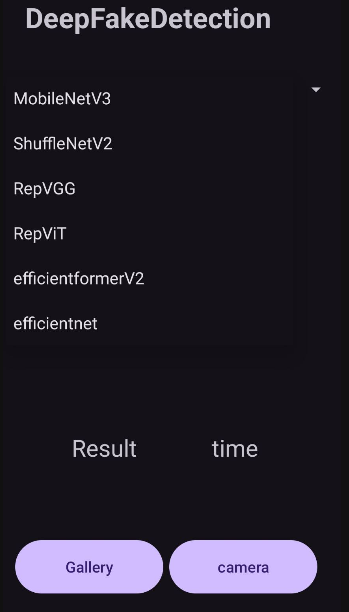
\includegraphics[width=0.75\linewidth]{figure/app_0.png}
    \caption{main page of the APP.}
    \label{fig:f2}
  \end{subfigure}
  \hfill
  \begin{subfigure}{0.45\linewidth}
    \centering
    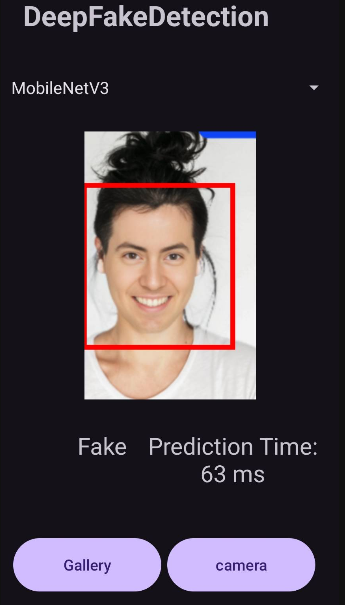
\includegraphics[width=0.75\linewidth]{figure/app_1.png}
    \caption{prediction showcase.}
    \label{fig:f3}
  \end{subfigure}
  \caption{Show case of the Android App.}
  \label{fig:f4}
\end{figure}

\section{Implemetation}
First, the FF++\cite{Rossler_2019_ICCV} dataset consists of five different methodologies, comprising 1,000 real videos and 5,000 fake videos. To balance the uneven distribution of the data, we extract five times more frames from the real videos, following the settings in \cite{qian2020thinking}. After that, we divide the 1000 original videos into 720 for training set 140 for validation set and 140 for testing set.
We selected six deep learning models: MobileNetV3\cite{howard2019searching}, ShuffleNetV2\cite{ma2018shufflenet},EfficientNet\cite{tan2020efficientnet}, EfficientFormer\cite{li2023rethinking} , RepVGG\cite{ding2021repvgg} and the state-of-the-art model, RepViT\cite{wang2024repvit}. The training recipe for these 6 models includes batch size 256, learning rate 0.001, adam optimizer\cite{kingma2017adam} with the pretrained\cite{rw2019timm} models on timm\cite{rw2019timm}.All of the models were trained for 25 epochs.

After completing the training, we built a simple Android app using Android Studio and Java. This deepfake detection app connects with PyTorch Mobile, allowing users to upload an image to determine whether it is real or fake. Before making a prediction, we use Google ML Kit to detect human faces in the picture and then crop the detected faces for prediction.

\section{Result}
~\cref{tab:acc} presents the test accuracy on both the FF++\cite{Rossler_2019_ICCV} and Celeb-DF-v2\cite{li2020celebdf} datasets. EfficientNet-B0\cite{tan2020efficientnet} and MobileNetV3-L\cite{howard2019searching} achieved the highest test accuracy, while RepViT\cite{wang2024repvit} showed the lowest accuracy, indicating its limitations in detecting deepfakes.

~\cref{tab:time} shows the inference time, number of parameters, and FLOPs for each model on an Android mobile device. ShuffleNetV2-1.5X\cite{ma2018shufflenet} and MobileNetV3-L\cite{howard2019searching} demonstrated faster inference times, making them suitable for real-time applications. EfficientNet-B0\cite{tan2020efficientnet}, while highly accurate, had a longer inference time, suggesting higher computational demands.

The training and validation performance of six models—MobileNetV3\cite{howard2019searching}, ShuffleNetV2\cite{ma2018shufflenet}, EfficientNet-B0\cite{tan2020efficientnet}, EfficientFormerV2\cite{li2023rethinking}, RepVGG\cite{ding2021repvgg}, and RepViT\cite{wang2024repvit}—are shown in~\cref{fig:f1}. MobileNetV3-L\cite{howard2019searching}, ShuffleNetV2\cite{ma2018shufflenet}, and EfficientNet-B0\cite{tan2020efficientnet} achieved high training and validation accuracy, with EfficientNet-B0\cite{tan2020efficientnet} slightly leading. RepVGG\cite{ding2021repvgg} and RepViT\cite{wang2024repvit} struggled with higher validation loss and lower validation accuracy, indicating challenges in generalization. 

~\cref{fig:f4} shows the design of the app. The image on the left depicts the app’s interface and the available models. The image on the right displays the results obtained after selecting a photo from the gallery, including the selected photo, prediction time, and prediction result. The red box in the photo indicates the face detection result.

\begin{table}[t]
\centering
\scalebox{1}{
\begin{tabular}{l| c| cc}
\toprule[0.2em]
Model & Test ACC & Celeb DF ACC   \\ 
\midrule
mobilenetV3-L    & 0.91 & 0.74  \\
ShuffleNetV2-1.5X     & 0.87 & 0.74  \\
efficientnet-B0 &  0.91 & 0.75 \\
efficientformerV2-S0 & 0.88 & 0.72  \\
RepVGG & 0.89 & 0.74  \\
RepViT & 0.69 & 0.72  \\
\bottomrule
\end{tabular}
}
\caption{Performance on both Df++ and Celeb DF V2}
\label{tab:acc}
\end{table}



\begin{table}[t]
\centering
\scalebox{0.8}{
\begin{tabular}{l| c| cc}
\toprule[0.2em]
Model & Inference time(s) & params(M) & FLOPs(M)   \\ 
\midrule
MobileNetV3-L &  41.1 & 5.48 & 438  \\
ShuffleNetV2-1.5X &  35.6  & 3.5 & 597  \\
efficientnet-B0 & 53.8 &  5.28 & 390 \\
efficientformerV2-S0 & 50.1  & 3.6 & 800  \\
RepVGG & 57.5 & 8.3 & 136 \\
RepViT & 65.2 & 6.8 & 220  \\
\bottomrule
\end{tabular}
}
\caption{Performance on android mobile device}
\label{tab:time}
\end{table}

\section{Conclusion}
This study underscores the complexities involved in deploying deepfake detection models on Android devices, highlighting the intricate trade-offs between model complexity, accuracy, and inference time. Among the models evaluated, EfficientNet-B0\cite{tan2020efficientnet} emerged as the most accurate on both the FF++\cite{Rossler_2019_ICCV} and Celeb-DF-v2\cite{li2020celebdf} datasets, showcasing its robustness in handling diverse deepfake scenarios. However, its longer inference time highlights the computational demands, which could restrict its practical application in real-time scenarios.

ShuffleNetV2-1.5X\cite{ma2018shufflenet} demonstrated an optimal balance, combining high accuracy with faster inference times, making it highly suitable for mobile applications where prompt responses are essential. Similarly, MobileNetV3-L, while slightly lagging behind in accuracy compared to ShuffleNetV2-1.5X\cite{ma2018shufflenet}, still offered a commendable trade-off between accuracy and speed.

EfficientFormerV2-S0\cite{li2023rethinking} presented competitive inference times but did not achieve top-tier accuracy, indicating room for improvement. RepVGG\cite{ding2021repvgg} and RepViT\cite{wang2024repvit}, despite showing promise during training on the FF++\cite{Rossler_2019_ICCV} dataset, revealed significant drops in accuracy on the Celeb-DF-v2\cite{li2020celebdf} dataset,  suggesting potential overfitting and challenges in generalizability.

Analyzing the training and validation performance in ~\cref{fig:f1} provided deeper insights into the learning dynamics of these models. MobileNetV3, ShuffleNetV2\cite{ma2018shufflenet}, and EfficientNet-B0\cite{tan2020efficientnet} not only achieved high accuracy but also demonstrated consistent performance across epochs, while RepVGG\cite{ding2021repvgg} and RepViT\cite{wang2024repvit} struggled with stability and generalization, as evidenced by higher validation loss and fluctuating accuracy.

The application design in~\cref{fig:f2} successfully integrates the model selection and prediction workflow, utilizing Google's ML Kit for initial face detection, which streamlines the preprocessing stage before deepfake verification. This design choice significantly enhances user experience and operational efficiency.

The results in~\cref{tab:acc} affirmed that EfficientNet-B0\cite{tan2020efficientnet} and MobileNetV3-L\cite{howard2019searching} led in accuracy, while RepViT\cite{wang2024repvit} lagged, indicating its limitations.~\cref{tab:time} highlighted that ShuffleNetV2-1.5X\cite{ma2018shufflenet} and MobileNetV3-L\cite{howard2019searching} had faster inference times, reinforcing their suitability for mobile platforms. EfficientNet-B0’s\cite{tan2020efficientnet} longer inference time, despite its accuracy, points to a need for further optimization.

In conclusion, the findings suggest that EfficientNet-B0\cite{tan2020efficientnet} and ShuffleNetV2-1.5X are the most promising candidates for mobile deepfake detection, each excelling in different aspects of performance. Future work should focus on refining these models to further enhance their efficiency and accuracy. Strategies may include reducing model complexity, optimizing algorithms for faster inference, and improving generalizability to unseen data. Additionally, continuous monitoring and adaptation to evolving deepfake generation techniques are imperative for maintaining the efficacy and reliability of detection systems in real-world applications. This holistic approach will ensure that deepfake detection on mobile platforms remains robust, accurate, and efficient, catering to the growing need for real-time verification tools.


%%%%%%%%% REFERENCES
{\small
\bibliographystyle{ieee_fullname}
\bibliography{egbib}
}

\end{document}
